\documentclass[border=4pt,12pt]{standalone}
% House style for redrawn exam diagrams (diagram-v4: 0.4pt lines, filled -latex arrows, fine dashes; stipple and hatching drawn as real dots/lines (no PDF/SVG patterns, so they render in every browser and at any scale); transparent background). Every figure \input's this.
\usepackage{amsmath,amssymb}
\usepackage{txfonts}
\usepackage{pdfrender,xcolor}
% \halo{text}: label on shading. The shading stops just around each letter's outline (a thin knock-out that follows the
% glyphs, like the papers' typesetting), never a box. Owner: "I don't want a box around the text".
\newcommand{\halo}[1]{\leavevmode\rlap{\pdfrender{TextRenderingMode=2,LineWidth=2.2pt,LineJoinStyle=1,StrokeColor=white,FillColor=white}#1}#1}
\usepackage{tikz,pgfplots}
\pgfplotsset{compat=1.18}
\usetikzlibrary{arrows.meta,calc,angles,quotes,patterns,patterns.meta,intersections,positioning,decorations.markings,shapes.geometric}
% Stipple and hatching are drawn as actual dots / lines clipped to the region (path picture), NOT as pattern fills:
% SVG <pattern> fills vanish or blur when browsers scale the image, so the owner could not see the shading.
% Each dot is a 0.72pt square (keeps SVGs small; reads as a dot at print size). Dots sit on one global staggered grid, so neighbouring regions line up.
\makeatletter
\newdimen\ex@x \newdimen\ex@y \newdimen\ex@xa \newdimen\ex@ya \newdimen\ex@xb \newdimen\ex@yb \newcount\ex@row
\def\exam@stipplecolor{black!75}\def\exam@dotr{0.42pt}\def\exam@dotgap{2.5}
\def\ex@rowdots{\ifdim\ex@x<\ex@xb \pgfpathrectangle{\pgfqpoint{\dimexpr\ex@x-0.36pt\relax}{\dimexpr\ex@y-0.36pt\relax}}{\pgfqpoint{0.72pt}{0.72pt}}\advance\ex@x by \exam@dotgap pt\relax\expandafter\ex@rowdots\fi}
\def\exam@stipple{%
  \pgftransformreset% dots are sized in real points even inside scaled pictures
  \pgfpointanchor{path picture bounding box}{south west}\ex@xa=\pgf@x \ex@ya=\pgf@y
  \pgfpointanchor{path picture bounding box}{north east}\ex@xb=\pgf@x \ex@yb=\pgf@y
  \pgfsetfillcolor{\exam@stipplecolor}\pgfmathsetmacro\ex@h{\exam@dotgap/2}%
  \pgfmathtruncatemacro\ex@r{floor(\ex@ya/\ex@h)-1}\ex@row=\ex@r\relax
  \ex@y=\ex@r\dimexpr\ex@h pt\relax
  \loop\ifdim\ex@y<\ex@yb
    \pgfmathtruncatemacro\ex@c{floor(\ex@xa/\exam@dotgap)-1}\ex@x=\ex@c\dimexpr\exam@dotgap pt\relax
    \ifodd\ex@row \advance\ex@x by \ex@h pt\fi
    \ex@rowdots
    \advance\ex@y by \ex@h pt \advance\ex@row by 1
    \ifnum\numexpr\ex@row-(\ex@row/4)*4\relax=0 \pgfusepath{fill}\fi% flush every 4 rows: bounded TeX memory, few clip copies in the SVG
  \repeat\pgfusepath{fill}}
\newdimen\ex@d
\def\exam@hatch#1{% #1 = 1 for /, -1 for \ ; lines 45 degrees, 3pt apart
  \pgftransformreset
  \pgfpointanchor{path picture bounding box}{south west}\ex@xa=\pgf@x \ex@ya=\pgf@y
  \pgfpointanchor{path picture bounding box}{north east}\ex@xb=\pgf@x \ex@yb=\pgf@y
  \ex@d=\dimexpr\ex@yb-\ex@ya\relax \ex@x=\dimexpr\ex@xa-\ex@d\relax
  \loop\ifdim\ex@x<\ex@xb
    \ifnum#1>0 \pgfpathmoveto{\pgfqpoint{\ex@x}{\ex@ya}}\pgfpathlineto{\pgfqpoint{\dimexpr\ex@x+\ex@d\relax}{\ex@yb}}%
    \else \pgfpathmoveto{\pgfqpoint{\ex@x}{\ex@yb}}\pgfpathlineto{\pgfqpoint{\dimexpr\ex@x+\ex@d\relax}{\ex@ya}}\fi
    \advance\ex@x by 4.24pt
  \repeat
  \pgfsetlinewidth{0.4pt}\pgfsetstrokecolor{black}\pgfusepath{stroke}}
\def\examstipple{\exam@stipple}\def\examhatch{\exam@hatch}\def\examsetstipplecolor#1{\def\exam@stipplecolor{#1}}\def\examsetdotgap#1{\def\exam@dotgap{#1}}
\makeatother
% (legacy pattern kept for old files)
% staggered stipple like the NESA papers' dotted shading
\pgfdeclarepatternformonly{exam stipple}{\pgfpointorigin}{\pgfqpoint{2.2pt}{2.2pt}}{\pgfqpoint{2.2pt}{2.2pt}}{%
  \pgfpathcircle{\pgfqpoint{0.55pt}{0.55pt}}{0.42pt}\pgfpathcircle{\pgfqpoint{1.65pt}{1.65pt}}{0.42pt}\pgfusepath{fill}}
\tikzset{
  every picture/.style={line width=0.6pt, >={Latex[length=2mm,width=1.3mm]}},
  curve/.style={line width=0.6pt},
  open arrow/.style={-{Latex[length=2mm,width=1.3mm]}},  % owner: filled -latex heads everywhere, no open chevrons
  aux/.style={dash pattern=on 2pt off 1.5pt, line width=0.6pt},
  shade/.code={\def\exA{#1}\def\exB{none}\ifx\exA\exB\else\pgfkeysalso{fill=black!18}\fi},
  shade/.default=on,
  shade dots/.style={fill=none, path picture={\examstipple}},
  stipple color/.code={\examsetstipplecolor{#1}},
  stipple gap/.code={\examsetdotgap{#1}},
  shade dense dots/.style={fill=none, stipple gap=1.6, path picture={\examstipple}},
  shade hatch/.style={fill=none, path picture={\examhatch{1}}},
  shade hatch reverse/.style={fill=none, path picture={\examhatch{-1}}},
  shade solid/.style={fill=black},
  pt/.style={circle, fill, inner sep=1.1pt},
  open pt/.style={circle, draw, fill=white, inner sep=1.1pt},
}
\pgfplotsset{
  exam axes/.style={axis lines=middle, axis line style={->}, xlabel={$x$}, ylabel={$y$},
    xlabel style={anchor=west}, ylabel style={anchor=south}, tick label style={font=\small},
    every axis plot/.append style={line width=0.6pt, black}, samples=200, clip=false,
    enlargelimits=false, axis on top},
}

\begin{document}
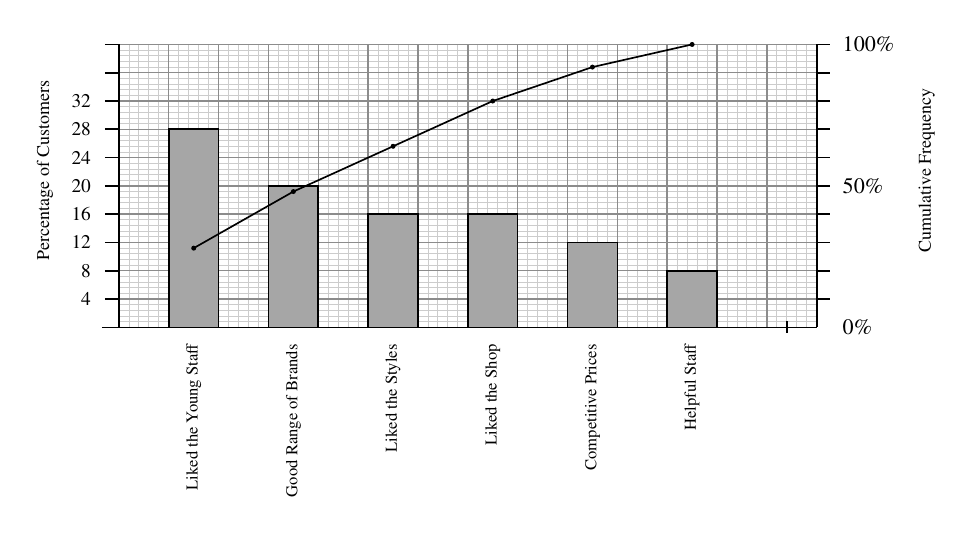
\begin{tikzpicture}[x=0.0127cm,y=-0.0127cm]
\def\CX#1{92+(#1)*49.857}
\def\PY#1{317-(#1)*7.075}
% minor grid
\foreach \i in {1,...,69}{\pgfmathtruncatemacro\m{mod(\i,5)}\ifnum\m=0\else
  \draw[black!20,line width=0.3pt] ({92+\i*9.971},34) -- ({92+\i*9.971},317);\fi}
\foreach \j in {1,...,49}{\pgfmathtruncatemacro\m{mod(\j,5)}\ifnum\m=0\else
  \draw[black!20,line width=0.3pt] (92,{317-\j*5.66}) -- (790,{317-\j*5.66});\fi}
% major grid
\foreach \c in {1,...,13}{\draw[black!45,line width=0.5pt] ({\CX{\c}},34) -- ({\CX{\c}},317);}
\foreach \v in {4,8,...,40}{\draw[black!45,line width=0.5pt] (92,{\PY{\v}}) -- (790,{\PY{\v}});}
% bars
\foreach \c/\h in {1/28,3/20,5/16,7/16,9/12,11/8}{
  \filldraw[fill=black!35,line width=0.6pt] ({\CX{\c}},317) rectangle ({\CX{\c+1}},{\PY{\h}});}
% axes
\draw (92,34) -- (92,317);
\draw (790,34) -- (790,317);
\draw (75,317) -- (790,317);
\draw (760,311) -- (760,323);
\foreach \v in {4,8,...,40}{\draw (78,{\PY{\v}}) -- (92,{\PY{\v}}); \draw (790,{\PY{\v}}) -- (803,{\PY{\v}});}
\foreach \v in {4,8,...,32}{\node[anchor=east,font=\fontsize{7}{8}\selectfont] at (74,{\PY{\v}}) {$\v$};}
\node[anchor=west,font=\fontsize{8}{9}\selectfont] at (806,{\PY{40}}) {$100\%$};
\node[anchor=west,font=\fontsize{8}{9}\selectfont] at (806,{\PY{20}}) {$50\%$};
\node[anchor=west,font=\fontsize{8}{9}\selectfont] at (806,{\PY{0}}) {$0\%$};
\node[rotate=90,font=\fontsize{6.5}{8}\selectfont] at (18,160) {Percentage of Customers};
\node[rotate=90,font=\fontsize{6.5}{8}\selectfont] at (900,160) {Cumulative Frequency};
\foreach \c/\t in {1/Liked the Young Staff,3/Good Range of Brands,5/Liked the Styles,7/Liked the Shop,9/Competitive Prices,11/Helpful Staff}{
  \node[rotate=90,anchor=east,font=\fontsize{6}{7}\selectfont] at ({\CX{\c+0.5}},324) {\t};}
% Pareto line
\draw ({\CX{1.5}},{317-0.28*283}) -- ({\CX{3.5}},{317-0.48*283}) -- ({\CX{5.5}},{317-0.64*283}) -- ({\CX{7.5}},{317-0.80*283}) -- ({\CX{9.5}},{317-0.92*283}) -- ({\CX{11.5}},{317-1.00*283});
\foreach \c/\p in {1.5/0.28,3.5/0.48,5.5/0.64,7.5/0.80,9.5/0.92,11.5/1.00}{\fill ({\CX{\c}},{317-\p*283}) circle (2.5);}
\end{tikzpicture}
\end{document}